\subsection*{Aufgabe 3 - Hennessy-Milner Logik: Modellierung}



$ (\Proc, \Act, \{ \CCSTrans{a} | a \in \Act \})$ \\
$ \Proc = \{p_1, p_2, p_3 \}$ \\
$ \Act = \{a, b, c, d\}$ \\
$ \CCSTrans{a} = \{ (p_1, p_2)\}$ \\
$ \CCSTrans{b} = \{ (p_2, p_1)\}$ \\
$ \CCSTrans{c} = \{ (p_2, p_2)\}$ \\
$ \CCSTrans{d} = \{ (p_1, p_3)\}$ \\

Es gilt:
$p_1 \models F_1 \land F_2 \land F_3 \land F_4 \land F_5$ \\

\begin{figure}[h!]
\begin{center}
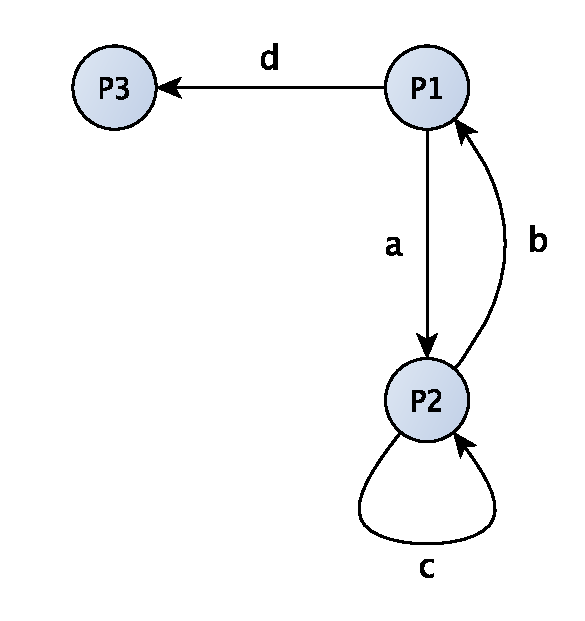
\includegraphics[width=13cm]{aufgabe3-lts}
%\caption{This is a figure.}
\end{center}
\end{figure}
